%-----------------------------------------------------------
%	Optimal loading paths
%-----------------------------------------------------------
\subsection{Optimal \textit{in silico} loading paths for parameter estimation}\label{sec:optimaldesign}

	Another technique for improving the parameter estimation process for determining $\Psi_{eff}$ from respective micro-models is establishing optimal loading paths. An example is the work of Avazmohammadi \cite{Avazmohammadi2017b}, where optimal experimental design is used to 1) minimize the amount of data necessary and 2) improve model parameter covariance for parameter estimation. Just like one of the most important question to ask before performing any mechanical testing is how much and what kind of data is necessary, we should also be selective with our choice of sampling points for parameter estimation. Theory for optimal design of experiment is a well-studied and documented \cite{lanir_optimal_1996, zhu_d_2014}. Vast majority of the methods for optimal design uses D-optimality as the design variable,
%==========================================================%
%-------------------	begin EQUATION 	-------------------%
\begin{equation}\label{eqn:doptimality}
\begin{aligned}
D = \det(\mathbfcal{I}), \quad \mathbfcal{I} = \mathbf{J}^\mathsf{T}\mathbf{J} \quad \mathrm{or} \quad \mathbfcal{I} = \mathbfcal{H},	\\
\mathrm{where} \ J_{ij} = \dpd{f_i}{\xi_j}, \quad \mathcal{H}_{ij} = \dmd{\mathcal{F}}{2}{\xi_i}{}{\xi_j}{},
\end{aligned}
\end{equation}
%-------------------	 end EQUATION 	-------------------%
%==========================================================% 
where $\mathbf{\xi}$ is a vector of model parameters, $\mathbfcal{I}$, the information matrix, can be computed from the derivatives of the objective function $\mathcal{F}$, where $f$ is the model evaluated at each data point, or $\mathbfcal{I}$ can be computed from the Hessian of the objective function, $\mathbfcal{H}$ (Appendix \ref{sec:parametercorrelation}). D-optimality, as the determinant of the information or the hessian matrix at best fit, offers the best representation of both parameter accuracy (parameter covariance or correlation) and precision (parameter variance) at the same time.

    
    The first and foremost step is to establish the parameterization for loading paths so they can be optimized. This is especially important and not straight a forward choice, as the number of loading paths required is not yet established. Another troubling this issue is that because the number of data points are discrete values, the D-optimality is typically not differentiable with respect to the control parameters. For the sake of time spent during optimization, the number of data points is to be kept at the minimal number necessary, thus exacerbating the issue of differentiability. Even worse is perhaps that the optimum is significantly better than the surrounding values, with non-optimal values essentially to zero. Unless the initial guess is near the optimum, optimization is very difficult. This of course means that conventional gradient algorithms are not practical for optimal design, requiring the need for Monte Carlo, random search or divide and conquer strategies, which are much more time consuming. 
    

%%%%%%%%%%%%%%%%%%%%%%%%%%%%%%%%%%%%%%%%%%%%%%%%%%%%%%%%%%%%
%-------------------	begin FIGURE 	-------------------%
\begin{figure}
\centering
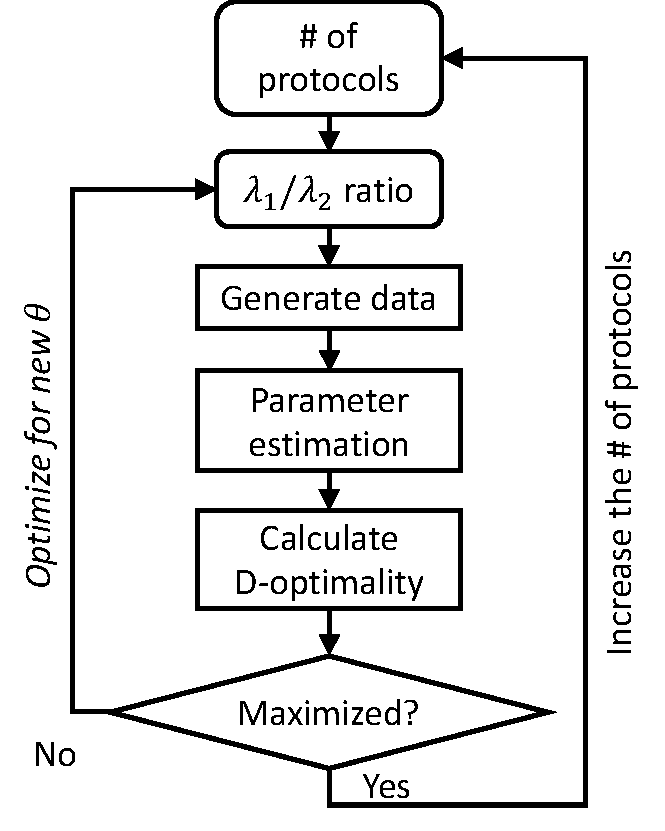
\includegraphics[width=3.25in]{Figures/optimaldesign}
\caption{Our approach for optimizing for the optimal loading paths for parameter estimation.}
\label{fig:optimaldesign}
\end{figure}
%-------------------	 end FIGURE 	-------------------%
%%%%%%%%%%%%%%%%%%%%%%%%%%%%%%%%%%%%%%%%%%%%%%%%%%%%%%%%%%%%

    
    We define loading paths based on the following conditions: 
\begin{enumerate}
\item The number of loading paths necessary
\item The number of variables needed to define a loading path and thus need to be iterated over
\item Possible application to mechanical testing of tissues.
\end{enumerate} 
Starting with planar extensions only, we chose a loading path as data points which shares the same stretch ratio, $\lambda_1/\lambda_2$, which is the same definition used for biaxial mechanical testing. This only requires one constant to be defined for each loading path and the resulting fan shape covers the largest range of deformation with the least number of data points. Next, with the total number of loading paths ranging from 1 to 6, we found 1) the total number of loading paths necessary before the benefit for adding additional loading paths is minimized and 2) the optimal ratio of the stretches for each of the individual loading path in the set (Fig. \ref{fig:optimaldesign}). Next the shear component is added. For each loading path, a parameter $\kappa_1$ for the maximum shear value reached is added to the same optimization framework (Fig. \ref{fig:optimaldesign}). For this case, we constrained the shear to be $0<\kappa_1<0.2$. Only the positive values of $\kappa_1$ is allowed due to the material symmetry. Furthermore, the optimal planar extensions loading paths are always incorporated into the dataset as a constant.



    

% %-----------------------------------------------------------
% %	Inverse parameter estimation
% %-----------------------------------------------------------
% \subsection{Inverse process for determining the parameter of high order models}

% 	The most crucial remaining question is whether the material parameters of complex downscale models can still be recovered from the response using the effective model. This is crucial for simulating time-dependent processes, which often requires recovering the material parameters of the downscale models to determine how the structural or material properties of the material parameters will change with time. For this, we compared the structural model parameter in two cases: 1) fitting the structural model to the experimental data, 2) fitting the effective model parameters to the experimental data, then fit the structural model to the response of the effective model. 
    
% %%%%%%%%%%%%%%%%%%%%%%%%%%%%%%%%%%%%%%%%%%%%%%%%%%%%%%%%%%%%
% %-------------------	begin FIGURE 	-------------------%
% \begin{figure}
% \centering
% \includegraphics[width=3.25in]{Figures/forwardinverseparameterestimation}
% \caption{Our approach testing how well the effective constitutive model can fully reproduce the mechanical response of soft tissues, and whether we can still recover the structural model parameter from the effective constitutive model.}
% \label{fig:forwardinverseparameterestimation}
% \end{figure}
% %-------------------	 end FIGURE 	-------------------%
% %%%%%%%%%%%%%%%%%%%%%%%%%%%%%%%%%%%%%%%%%%%%%%%%%%%%%%%%%%%%